\documentclass{standalone}
%% Show/hide steps for standalone work — edit this line:
\makeatletter\AtBeginDocument{\@buildstepset{1,2,3,4}}\makeatother
\usepackage{tikz}
\usepackage{hsbcommon}
\begin{document}
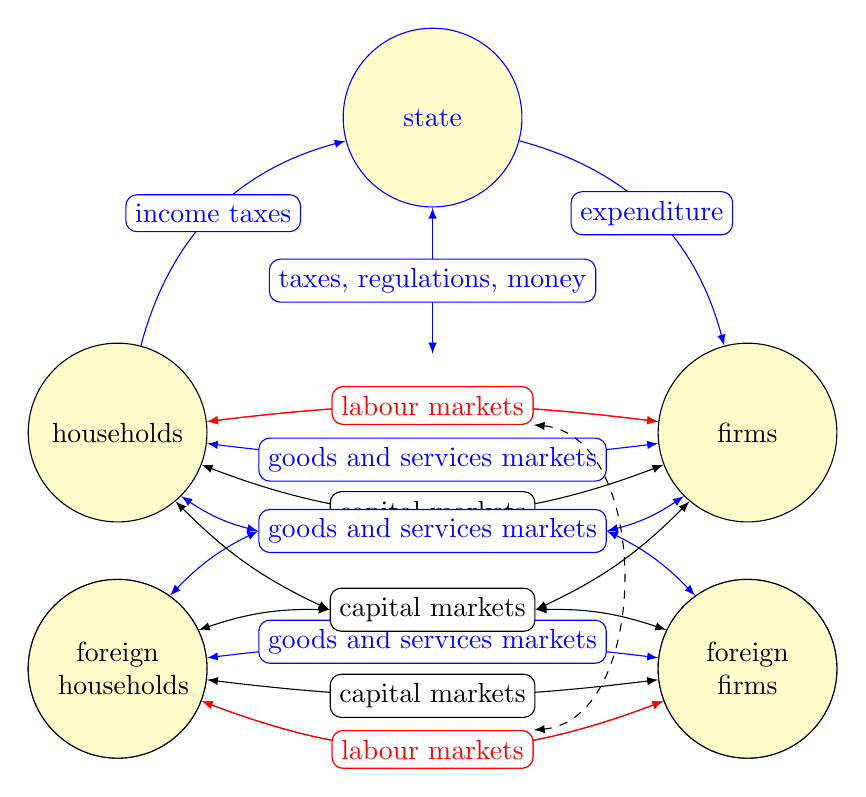
\begin{tikzpicture}[yscale=-1]
    \tikzset{%
        first/.style={draw, fill=yellow!20, circle, rounded corners,
            minimum width=15ex, minimum height=15ex},
        second/.style={draw, circle, minimum width=20ex},
        conn/.style={draw, rounded corners, fill=white},
        every path/.style={draw, >=latex}
    }
    \node[first] (HH) at (-4,0) {households};
    \node[first] (BN) at (4,0)  {firms};
    \phantom{    
        \node[first] (HHaus) at (-4,3) {households};
        \node[first] (BNaus) at (4,3)  {firms};
    }

    %% Step 1: internal markets
    \ifsteponly{1}{4}{
        \begin{scope}
            \draw[<->,bend left=7,color=blue] (HH) to node[conn] {goods and services markets}   (BN);
            \draw[<->,bend right=7,color=red]   (HH) to  node[conn] {labour markets}  (BN);
            \draw[<->,bend left=21,color=black]   (HH) to node[conn] {capital markets}  (BN);
        \end{scope}
    }


    %% Step 2: state
    \ifstep{2}{
        \begin{scope}[color=blue]
            \node[first] at (0,-4) (ST) {state};
            \draw[->,bend right=30] (HH) to node[conn,name=taxone] {income taxes}  (ST);
            \draw[->,bend right=30] (ST) to node[conn] {expenditure}    (BN);
            \draw[<->] (ST) -- node[conn,name=taxtwo] {taxes, regulations, money} (ST |-, -1);
            % \node[conn,fill=blue!10,draw=black] at (3,-6) {fiscal and regulatory policy};
        \end{scope}
    }

    %% Step 3: foreign country

    \ifsteponly{3}{4}{
        \begin{scope}
         \node[first] at (-4,3) {\parbox{10ex}{\centering foreign\\ households}};
        \node[first] at (4,3)  {\parbox{10ex}{\centering foreign\\ firms}};
            \draw[<->,bend right=7,color=blue] (HHaus) to node[conn] {goods and services markets}   (BNaus);
            \draw[<->,bend left=7,color=black]   (HHaus) to node[conn] {capital markets}  (BNaus);
            \draw[<->,bend left=21,color=red]   (HHaus) to coordinate (labwto) node[conn] {labour markets}  (BNaus);            
        \end{scope}        
    }

    %% Step 4: markets combine

    \ifstep{4}{
        \node[first] at (-4,3) {\parbox{10ex}{\centering foreign\\ households}};
        \node[first] at (4,3)  {\parbox{10ex}{\centering foreign\\ firms}};
        \draw[<->,bend left=21,color=red]   (HHaus) to node[conn,name=labone] {labour markets}  (BNaus);
        \draw[<->,bend right=7,color=red]   (HH) to node[conn,name=labtwo] {labour markets}  (BN);        

        \begin{scope}[blue]
            \node[conn] (newgoods) at (0,1.25) {goods and services markets};
            \draw[<->,bend left=10] (HH) to (newgoods.west);
            \draw[<->,bend left=10] (newgoods.west) to (HHaus);
            \draw[<->,bend right=10] (BN) to (newgoods.east);
            \draw[<->,bend right=10] (newgoods.east) to (BNaus);
        \end{scope}
        
        \begin{scope}[black]
            \node[conn,draw=black] (newcapital) at (0,2.25) {capital markets};
            \draw[<->,bend left=10] (HH) to (newcapital.west);
            \draw[<->,bend left=10] (newcapital.west) to (HHaus);
            \draw[<->,bend right=10] (BN) to (newcapital.east);
            \draw[<->,bend right=10] (newcapital.east) to (BNaus);
        \end{scope}

        \draw[<->, dashed,bend left=85] (labone.north east) to (labtwo.south east);
    }

    
\end{tikzpicture}
\end{document}

